\chapter{InterPlanetary File System
	\label{ch:InterPlanetary File System}}

The \textbf{Interplanetary File System} is a protocol and network designed to create a content-addressable, peer-to-peer method of storing and sharing hypermedia in a distributed file system. IPFS is a peer-to-peer distributed file system that seeks to connect all computing devices with the same system of files.
\section{IPFS Working}
In the figure below (see \figref{ipfs1}) shows an example of a person name jon who want to send a file using \textbf{IPFS}. By using \textbf{IPFS} File would be convert into \textbf{Hash} that would upload in InterPlanetary File System. 


\begin{figure}[h]
	\centering
	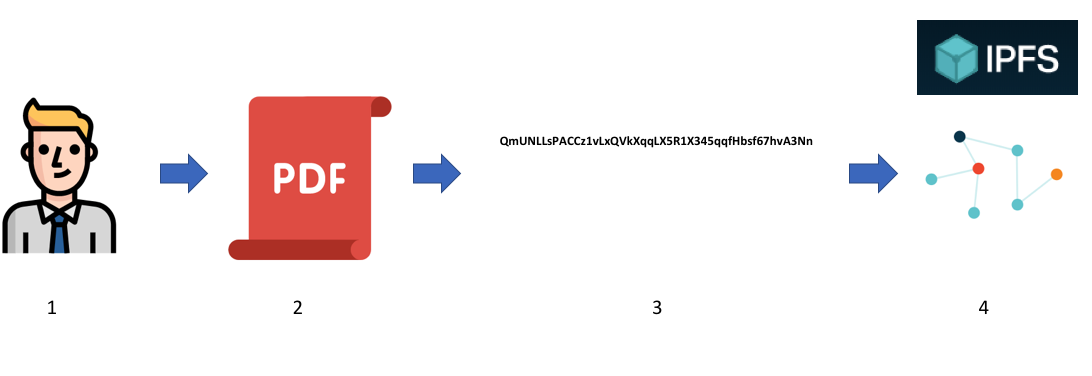
\includegraphics[width=450px]{figures/IPFS/10.png}
	\caption{IPFS File Upload}
	\label{fig:ipfs1}
\end{figure}

When Another Person name Sky want to Access that file just use \textbf{Hash} in InterPlanetary File System that give permission to Sky 
when \textbf{Hash} would match that upload in InterPlanetary File System see  the figure below (see \figref{ipfs2}) shows an example of Sky who Access that File.

\begin{figure}[h]
	\centering
	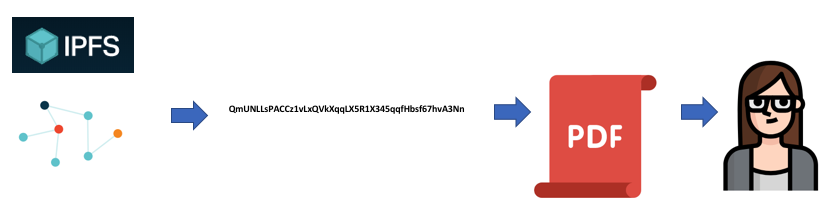
\includegraphics[width=450px]{figures/IPFS/11.png}
	\caption{IPFS File Access}
	\label{fig:ipfs2}
\end{figure}

IPFS would be same as BlockChain Network. When a File would be upload it turn on the Security that would not be Hacked the figure below (see \figref{ipfs3}) shows if Hash was Right file would be Access otherwise not Access-able. 
\begin{figure}[h]
	\centering
	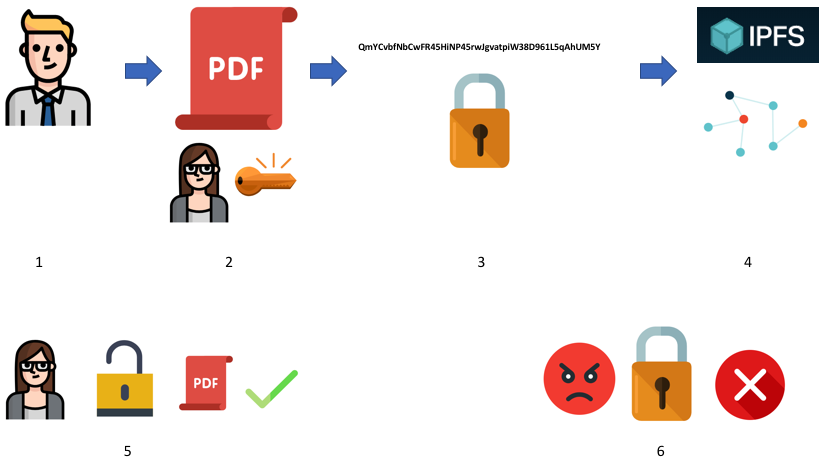
\includegraphics[width=450px]{figures/IPFS/12.png}
	\caption{IPFS File Access}
	\label{fig:ipfs3}
\end{figure}


\section{Installation}
\subsection{Install IPFS}
First of all install IPFS from their offical site that would be shown below.

\begin{figure}[h]
	\centering
	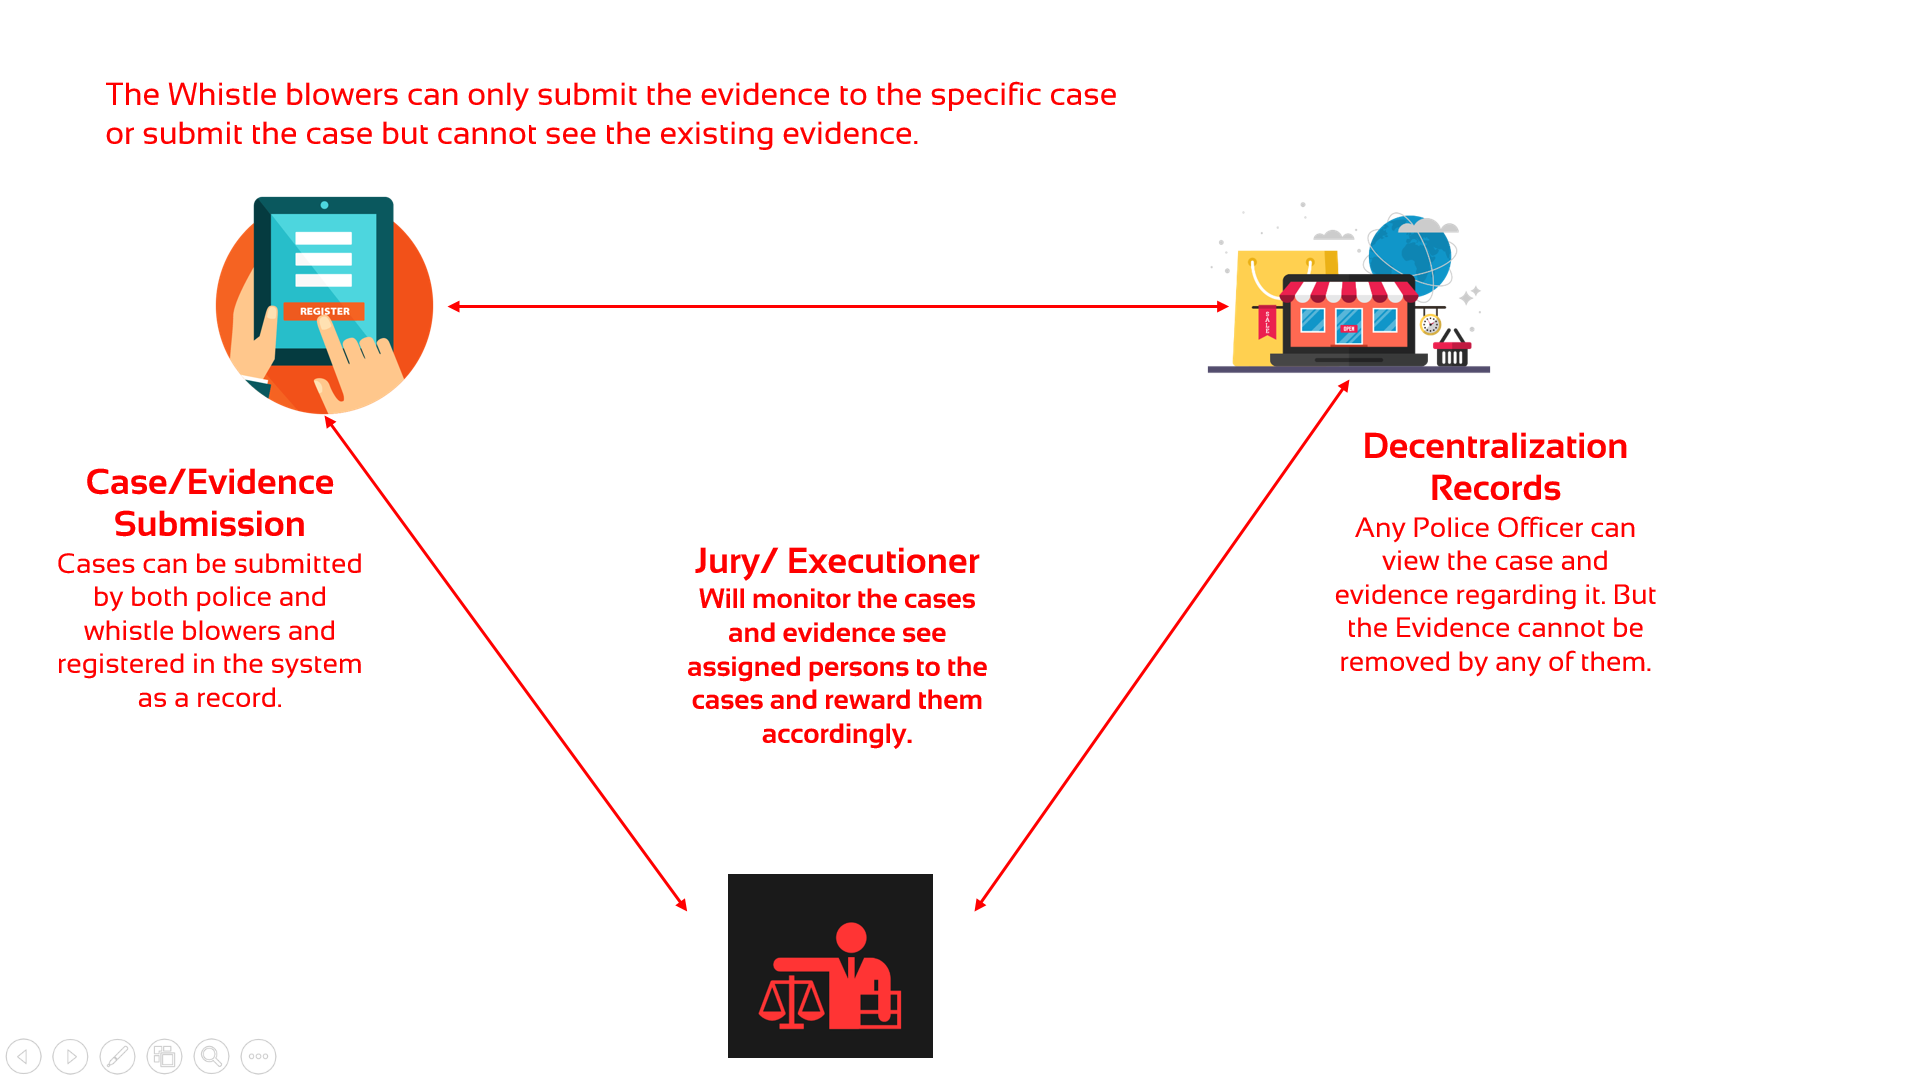
\includegraphics[width=450px]{figures/IPFS/01.png}
\end{figure}

\subsection{Editor}
You can use whatever editor you want we recommend using \textbf{Visual Studio Code} where we Attach \textbf{IPFS API} with \textbf{React}.
\newpage
\section{IPFS Update}
\subsection{Installing with IPFS-Update}
The Below figure shows IPFS-Updation
\begin{figure}[h]
	\centering
	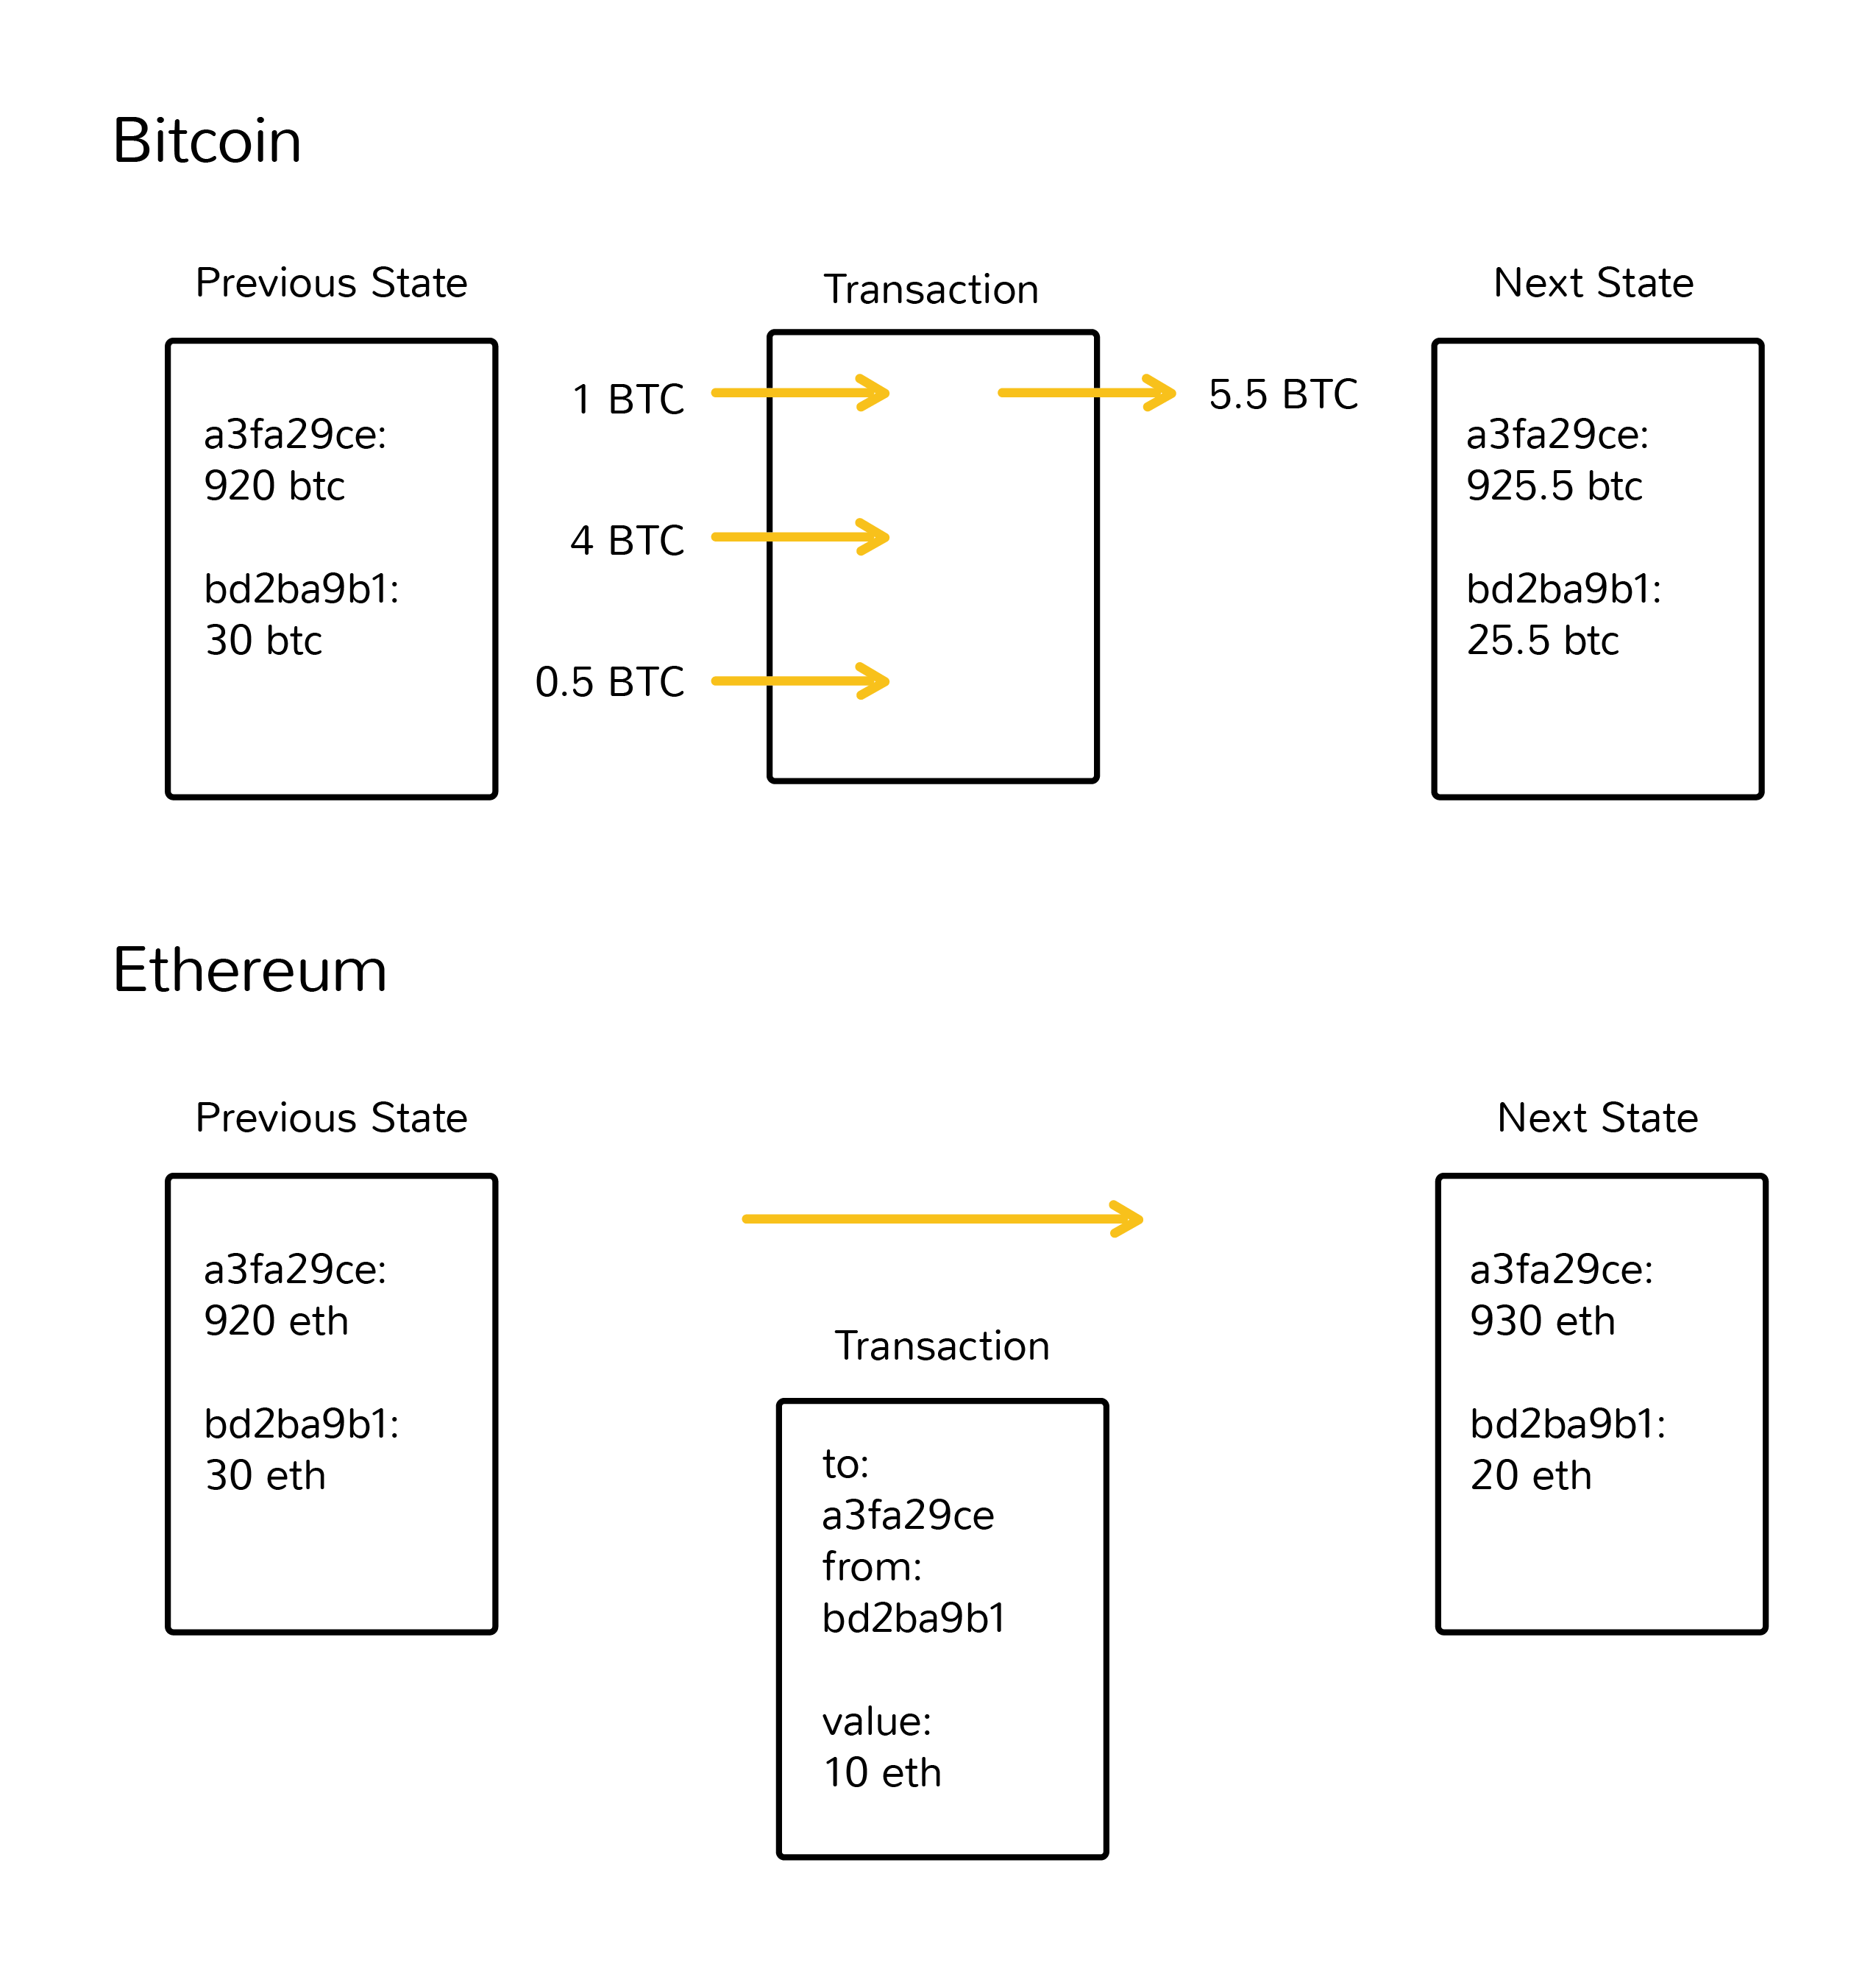
\includegraphics[width=450px]{figures/IPFS/02.png}
	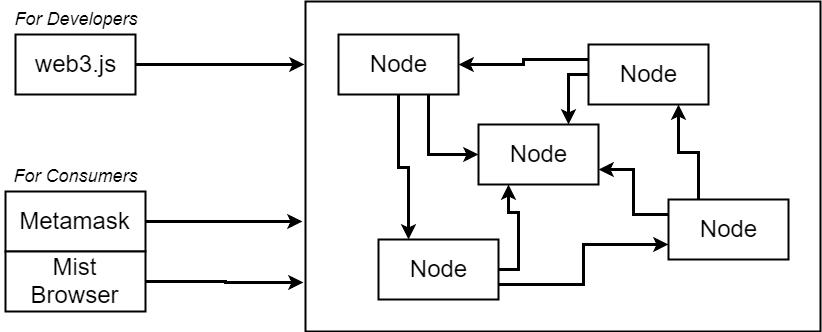
\includegraphics[width=450px]{figures/IPFS/04.png}
	
\end{figure}

\section{IPFS Repository}
\subsection{Initialize the repository}
IPFS stores all its settings and internal data in a directory called the repository. Before using IPFS for the first time, you’ll need to initialize the repository with the \textbf{ ipfs init} command The Below figure shows IPFS-Repository
\begin{figure}[h]
	\centering
	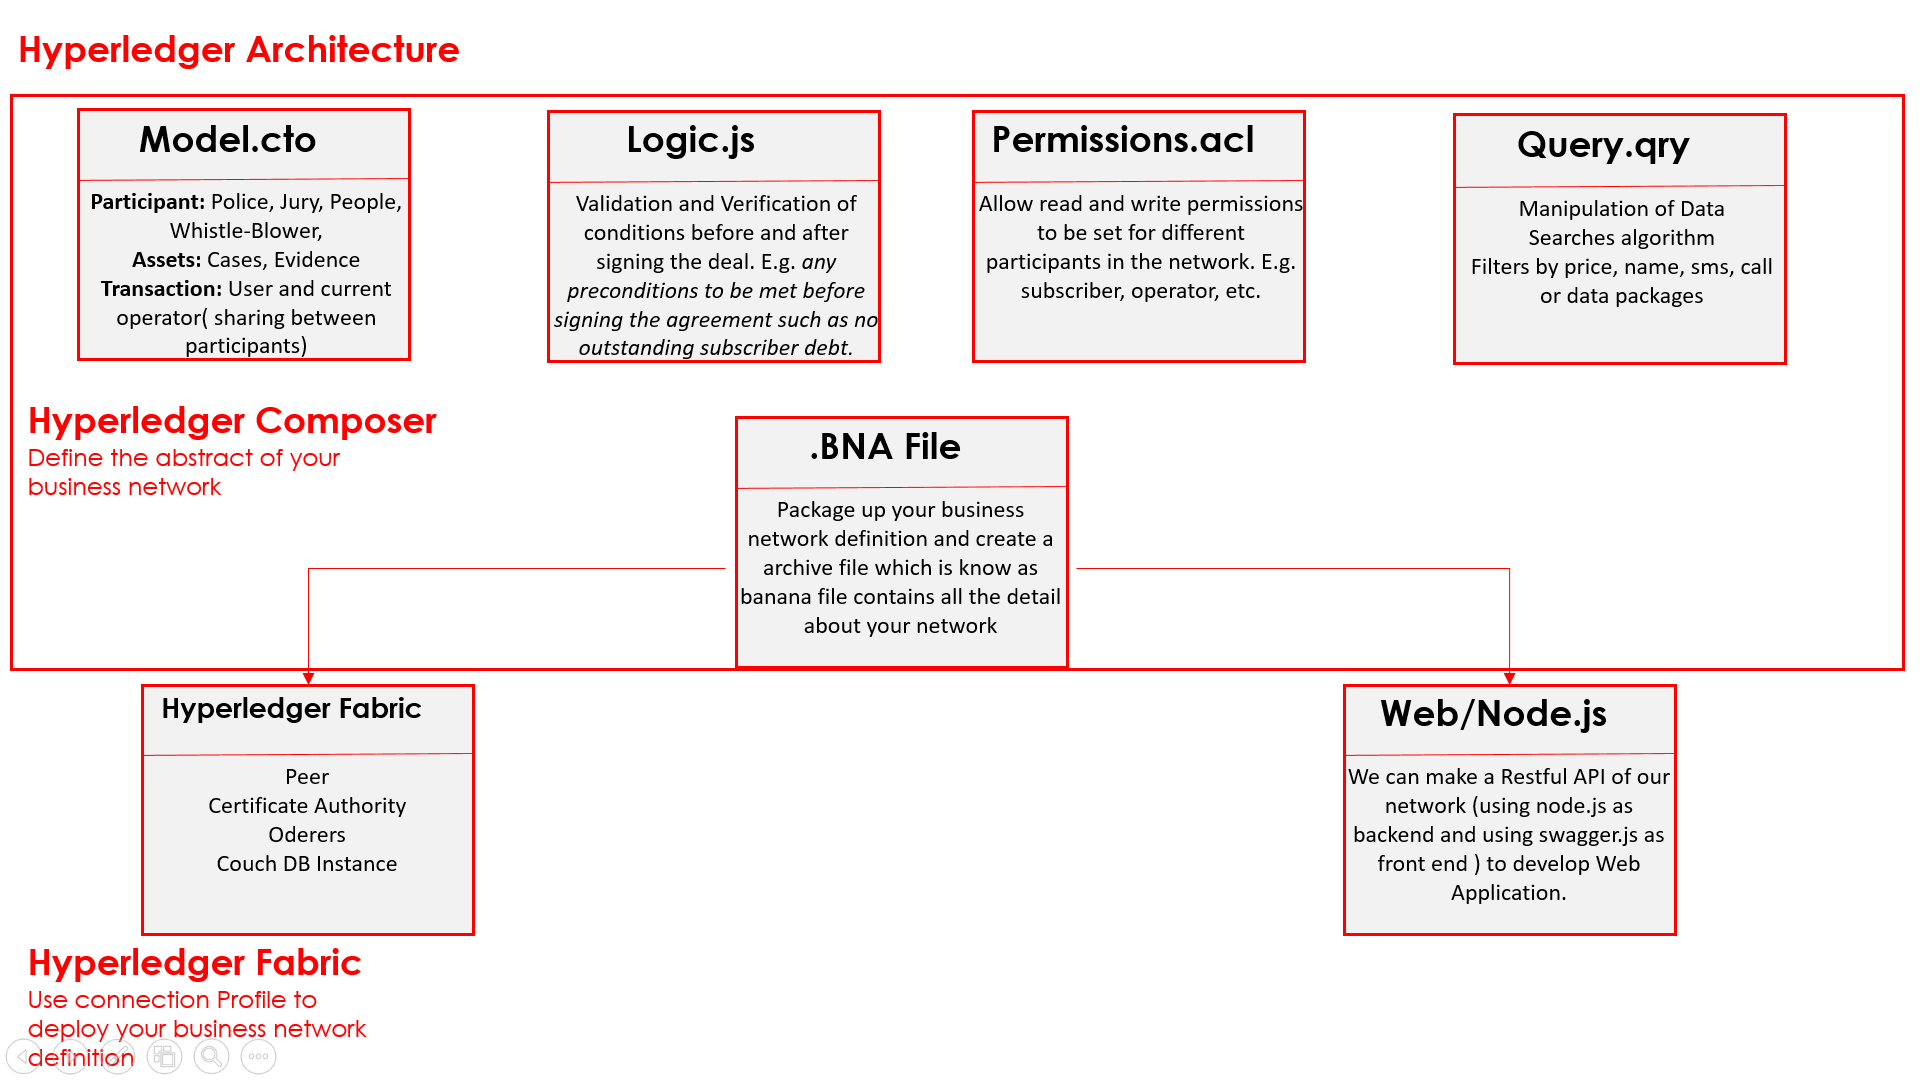
\includegraphics[width=450px]{figures/IPFS/05.png}
\end{figure}

Now, try running the command suggested to you in the output of ipfs init. The one that looks like \textbf{ipfs cat /ipfs/<HASH>/readme}.
You get Something like that show below
\begin{figure}[h]
	\centering
	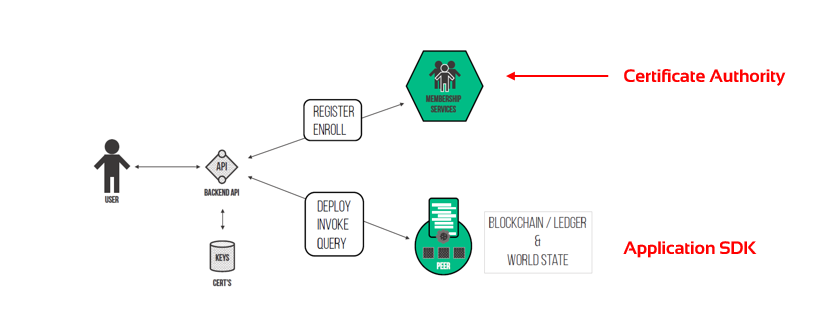
\includegraphics[width=310px]{figures/IPFS/06.png}
	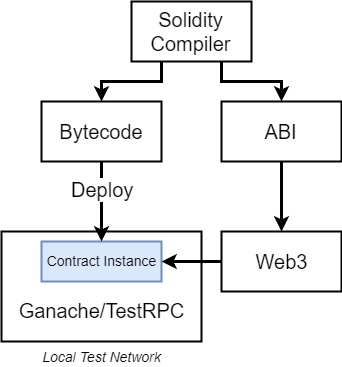
\includegraphics[width=310px]{figures/IPFS/09.png}
\end{figure}
\newpage
These steps can install your IPFS. Now for Check you can upload a hash using  (see \figref{ipfs7})

\begin{figure}[h]
	\centering
	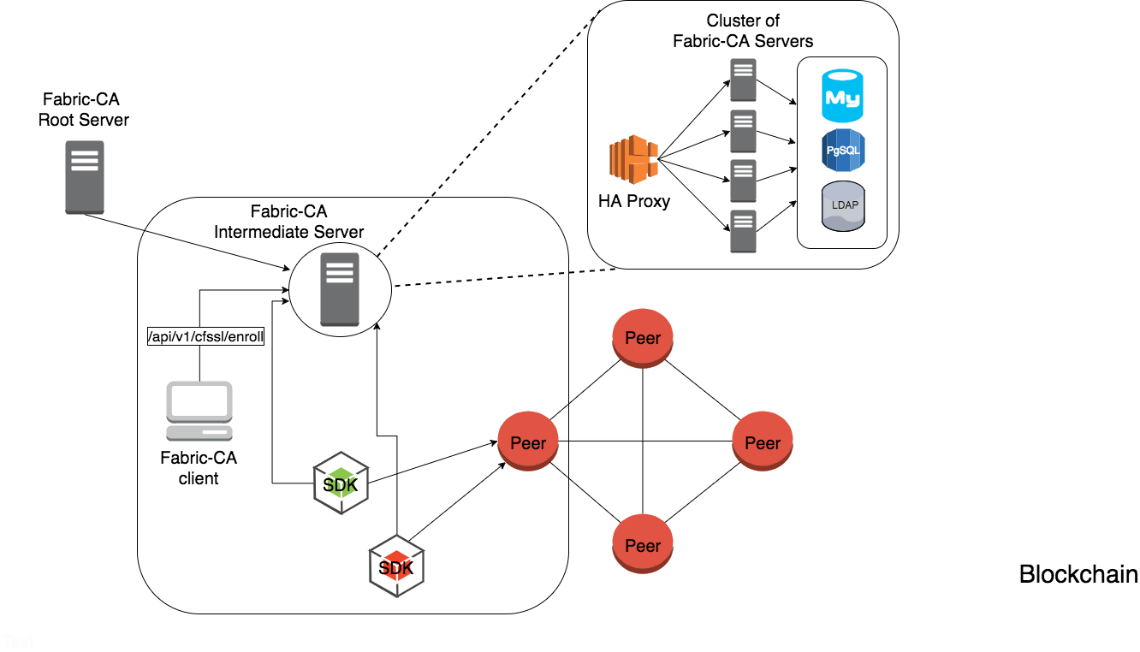
\includegraphics[width=450px]{figures/IPFS/07.png}
	\caption{Upload Hash}
	\label{fig:ipfs7}
\end{figure}

When we Check our File that Upload in IPFS you can use same hash using (see \figref{ipfs8}) in Command line.
\begin{figure}[h]
	\centering
	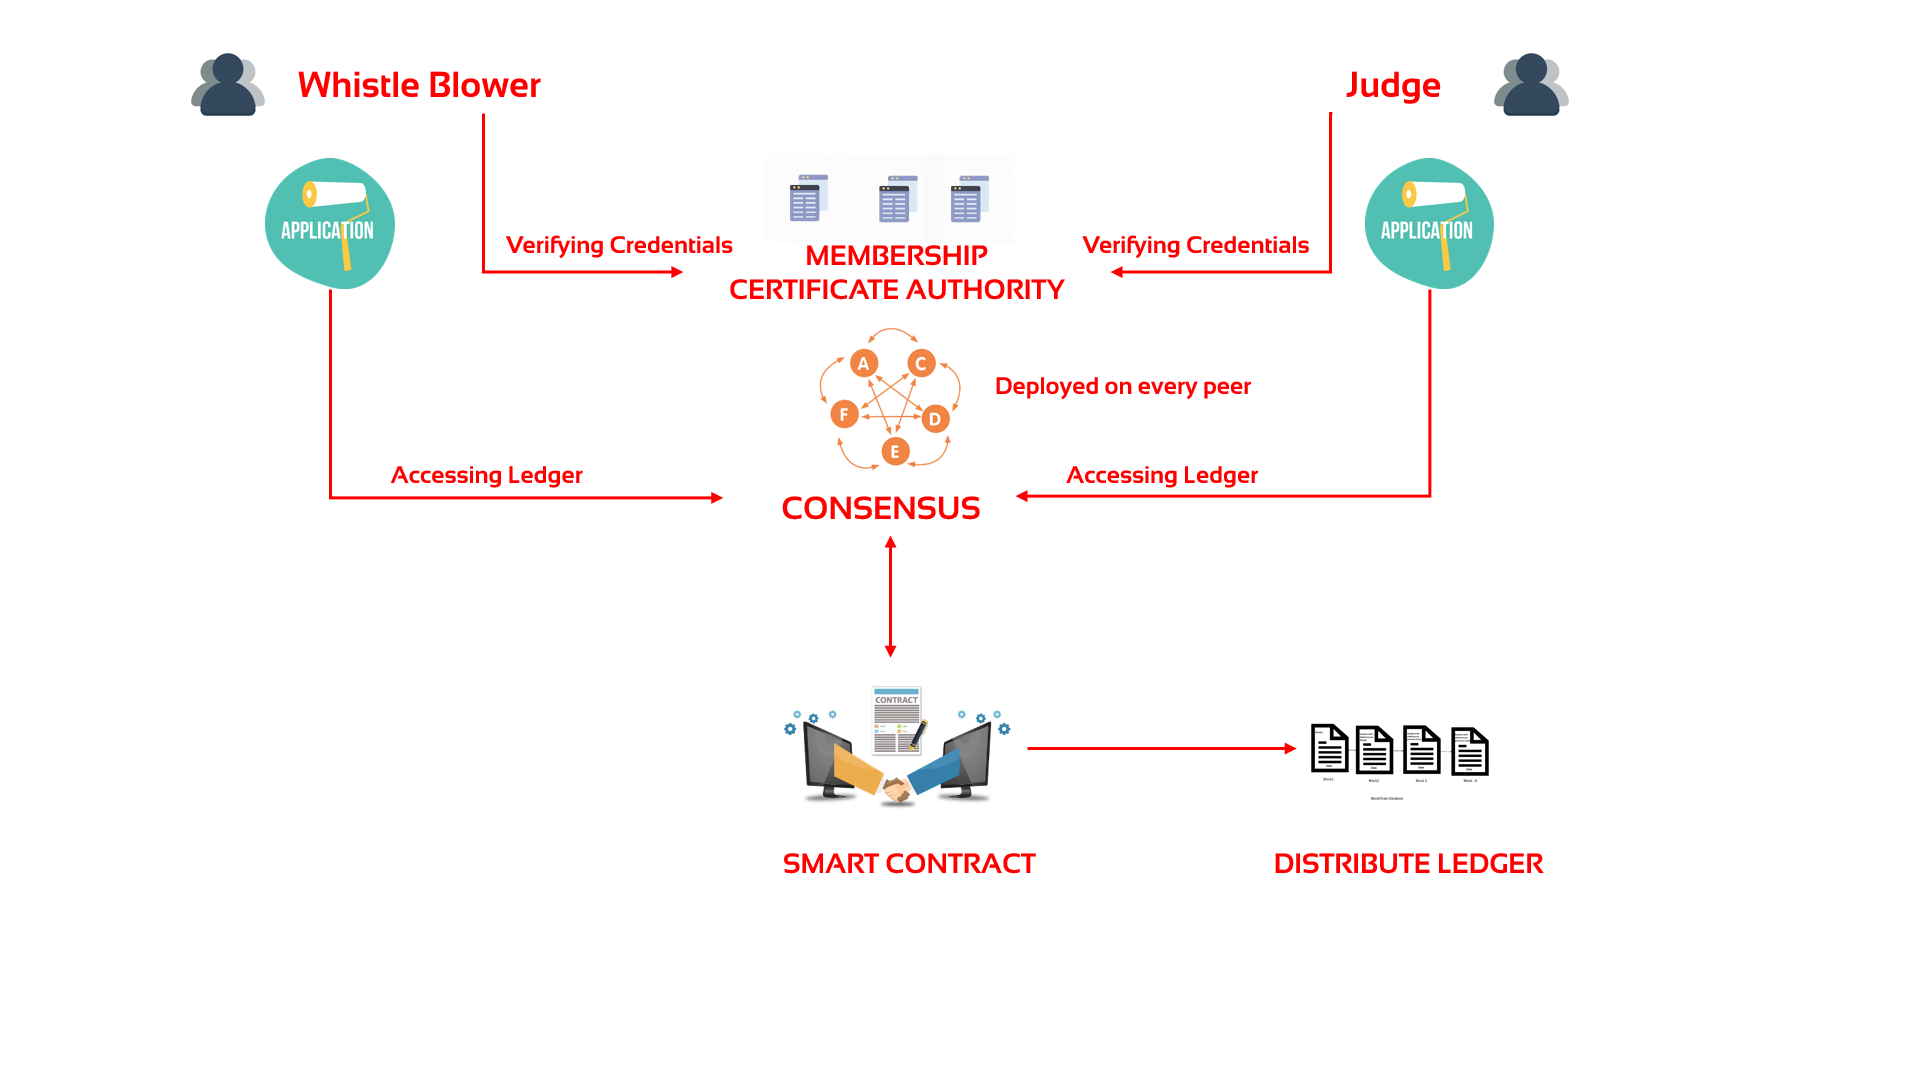
\includegraphics[width=450px]{figures/IPFS/08.png}
	\caption{Get Hash}
	\label{fig:ipfs8}
\end{figure}